% Nowcasting European LNG send-out from free public data
% SKELETON — structure, tables and claims are in place with real numbers;
% every \todo{} is prose or derivation that must be written by Solomon.
% Build: pdflatex main.tex (no exotic packages).
\documentclass[11pt]{article}
\usepackage[margin=1.1in]{geometry}
\usepackage{amsmath,amssymb,booktabs,graphicx,hyperref,xcolor}
\newcommand{\todo}[1]{\textcolor{red}{\textbf{[TODO-SOLOMON:} #1\textbf{]}}}
\title{Nowcasting European LNG send-out from free public data:\\
measured revision processes, calibrated filtering,\\ and a physical stress index}
\author{Solomon J.\ Williams\\ \small University of Edinburgh}
\date{Autumn 2026 — draft}

\begin{document}
\maketitle

\begin{abstract}
\todo{150 words. Claims to compress: (i) commercial-grade LNG supply signal
rebuilt entirely from free public sources, with the two layers vendors do not
publish — the revision process of the official data and calibrated
uncertainty; (ii) a semi-Markov, Rao-Blackwellized particle filter whose
evening nowcasts are 3--7$\times$ more accurate than any daily baseline with
distribution-free coverage guarantees; (iii) empirical findings en route:
official nominations are worse than persistence, the official intraday
estimate appears to be a carry-forward, intraday deviations are one random
ramp (fBm bridge $\hat H \approx 0.98$), arrivals are emphatically
non-Poisson; (iv) a days-of-cover stress index that adds AUC over storage
fullness in-sample, presented with its caveats.}
\end{abstract}

\section{Introduction}
\todo{2 pages. Outline: LNG send-out as a price-relevant hidden variable;
vendors sell it from proprietary satellite AIS; thesis = the open
reconstruction plus what vendors skip (revisions, calibration); contributions
list mirroring the abstract; related work in three strands — vessel-ETA
prediction (statistical/ML taxonomies, no stochastic-process treatment),
maritime inventory routing (prescriptive, import-terminal inventories
under-modelled, uncertainty ``in its infancy''), LNG arbitrage economics
(damped spread response). Cite the deep-research-verified sources.}

\section{Data: five free sources and their measured behaviour}
\todo{Prose around Table~\ref{tab:sources}; the measured-timing findings are
the section's substance — each was verified live and several contradict the
platforms' documentation.}
\begin{table}[h]\centering\small
\begin{tabular}{lllp{4.6cm}}
\toprule
Source & Access & Cadence & Measured behaviour \\
\midrule
ENTSOG transparency & keyless & daily/hourly & daily D $\to$ 09:20 D+1; hourly $\sim$2\,h lag; nominations for D at 16:00 D$-$1; UK rows backfilled $\sim$6\,d; some queries hang with zero bytes \\
GIE ALSI & free key & daily & 19:30 + 23:00 publications; dual-unit inventory (V13); UK absent since $\ge$2024; intraday E-row $=$ previous day's C (carry-forward; preliminary) \\
National Gas portal & keyless & daily + 2-min & D+1 physical at 12:01; D+2/M+15 ladder; per-sub-terminal 2-minutely instantaneous flows (not archived by the operator) \\
aisstream.io AIS & free key & streaming & terrestrial only; destination fields $\sim$52\% erroneous (lit.); berth calls resolvable; receiver gaps at Milford Haven/Dunkerque \\
AGSI / prices & free key / open & daily & EU storage aggregate; UK SAP; (TTF via Yahoo, analysis only) \\
\bottomrule
\end{tabular}
\caption{Sources and live-measured timing. \todo{tighten wording; add access dates.}}
\label{tab:sources}
\end{table}

\section{The revision processes of the official data}
\subsection{The UK ladder, reconstructed retroactively}
\todo{Prose: latestFlag=N serves every historical published version.
Findings: 27.8\% of values republished at $\sim$30 d with median change zero;
heavy tail to 662.7 GWh (send-out) and 340 GWh (stock, next-day); the
``M+15'' rung publishes at $\sim$M+1 and never differs from final D+2 (max
$\Delta$ = 0.00 over 2{,}829 matched days); D+1 physical $\approx$ final on
99\%+ of days (p99 0.02 GWh). Showcase: Grain 2025-04-21 — physical and
ENTSOG record $\sim$662 GWh, commercial retracted to 0 a month later; the
official record permanently self-contradicts, and that day's D+1 published
three days late.}
\subsection{The EU intraday estimate}
\todo{Carry-forward finding with the snapshot-archive methodology; state the
evidence window honestly (n days at time of writing) and the implication:
the official platform's intraday row carries no information, so an
ENTSOG-hourly nowcast is ahead by construction.}

\section{Cargo arrivals from mass balance}
\todo{Derive $A_t = \Delta I_t + S_t$; describe clustering; then:}
\begin{table}[h]\centering\small
\begin{tabular}{lccc}
\toprule
& median event (GWh) & 172k-class reference & deviation \\
\midrule
Dunkerque & 1095 & 1096 & $-0.1\%$ \\
Gate & 1105 & 1096 & $+0.8\%$ \\
Zeebrugge & 1096 & 1096 & $0.0\%$ \\
Montoir & 1092 & 1096 & $-0.4\%$ \\
\bottomrule
\end{tabular}
\caption{1{,}446 extracted arrivals; EU medians vs.\ the vessel-class
discharge energy implied by independent physics (capacity $\times$ fill
$\times$ boil-off $\times$ heel $\times$ GCV).}
\end{table}
\todo{Renewal structure: empirical hazard is exactly zero at 1-day gaps at
every terminal (berth turnaround); rising hazards at scheduled terminals
(Gate 0.56 by day 8). Dragon's staged discharges; multi-berth chaining.
Connect to the U6 arrival-hazard filter input.}

\section{A semi-Markov, Rao-Blackwellized nowcaster}
\todo{The model section — yours entirely. Content that must appear:
(i) explicit-duration regimes with NB sojourns as first-passage laws
(motivate hazard shapes from noise-induced escape); (ii) conditional
linear-Gaussianity and the marginalized filter, idle as the exact $S=0$
boundary state; (iii) the bridge observation model for intraday cumulatives
and the empirical kernel finding: fBm-bridge $\hat H \approx 0.98$ at all
hourly terminals ($-81$ to $-87\%$ correlation misfit vs Brownian) — one
random ramp factor per day; (iv) PGAS parameter posteriors, the
identifiability lessons (prior-tethering of unidentified sojourn blocks;
mixture label ordering), and parameter uncertainty in the bands.}

\begin{figure}[t]\centering
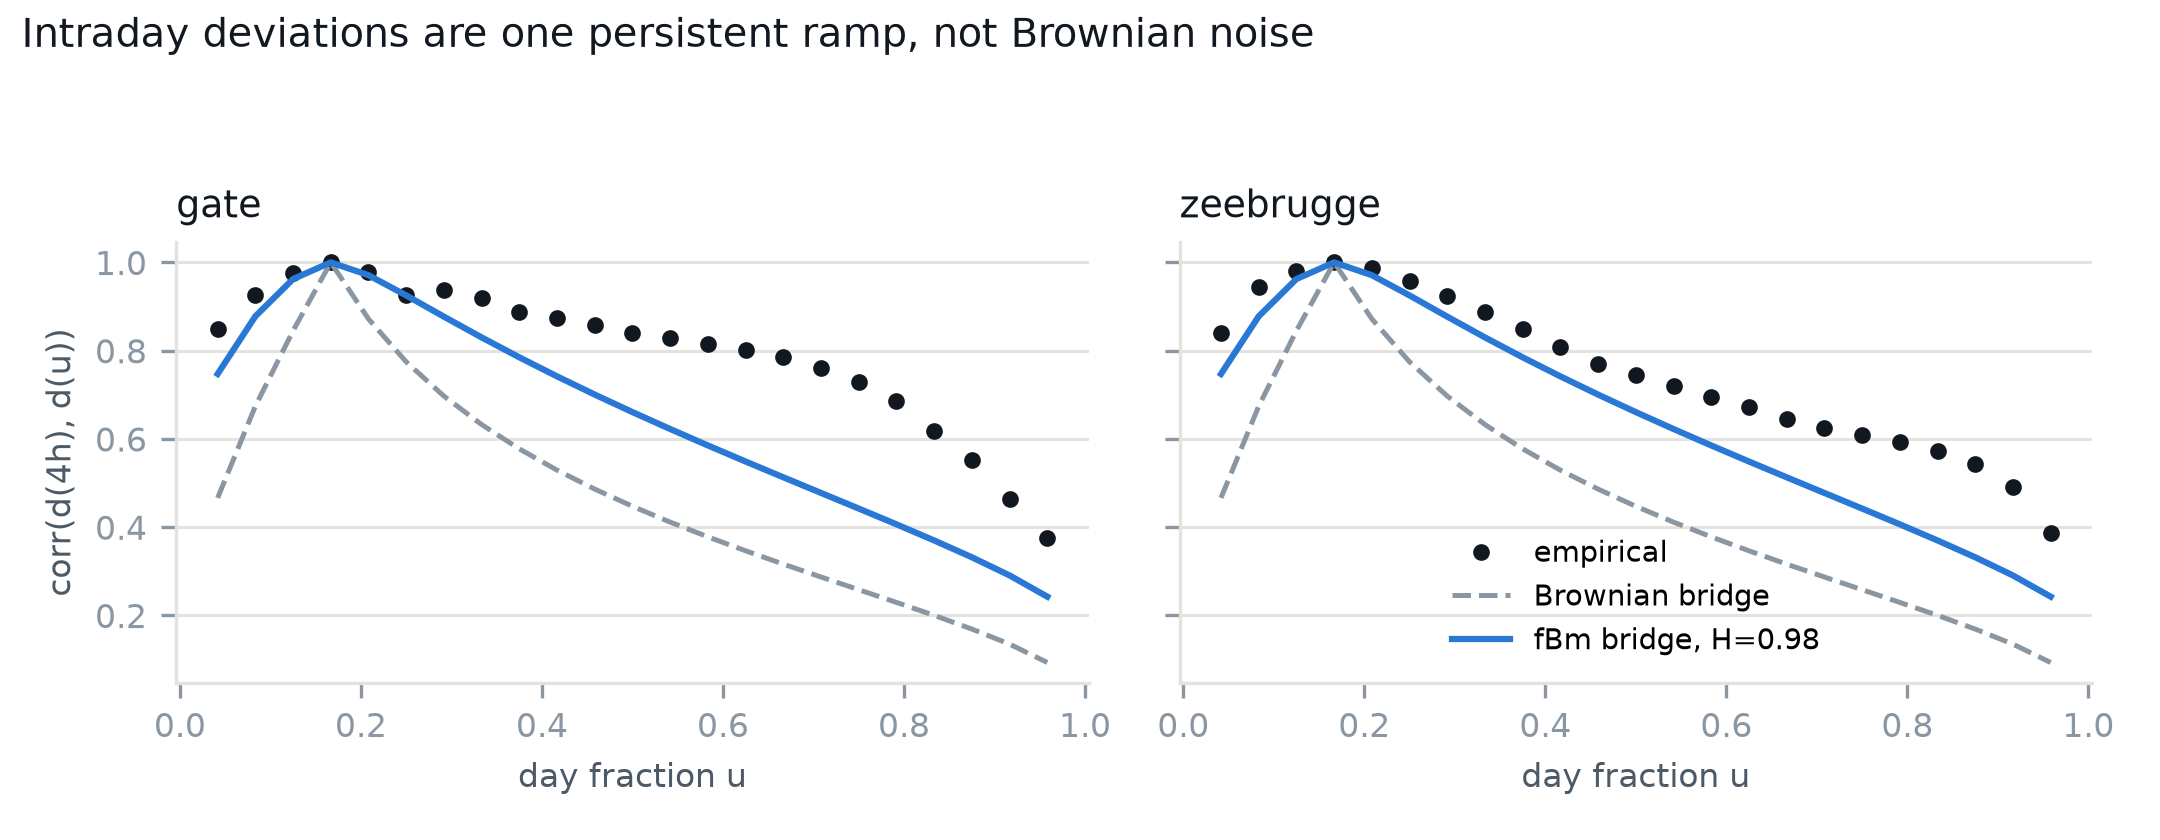
\includegraphics[width=\linewidth]{figures/fig_kernel.png}
\caption{Correlation of intraday deviations $d(u)$ with the hour-4 value:
the empirical structure (dots) tracks a fractional-Brownian bridge with
$H=0.98$, far from Brownian. \todo{caption polish.}}
\end{figure}

\section{Walk-forward evaluation}
\begin{figure}[t]\centering
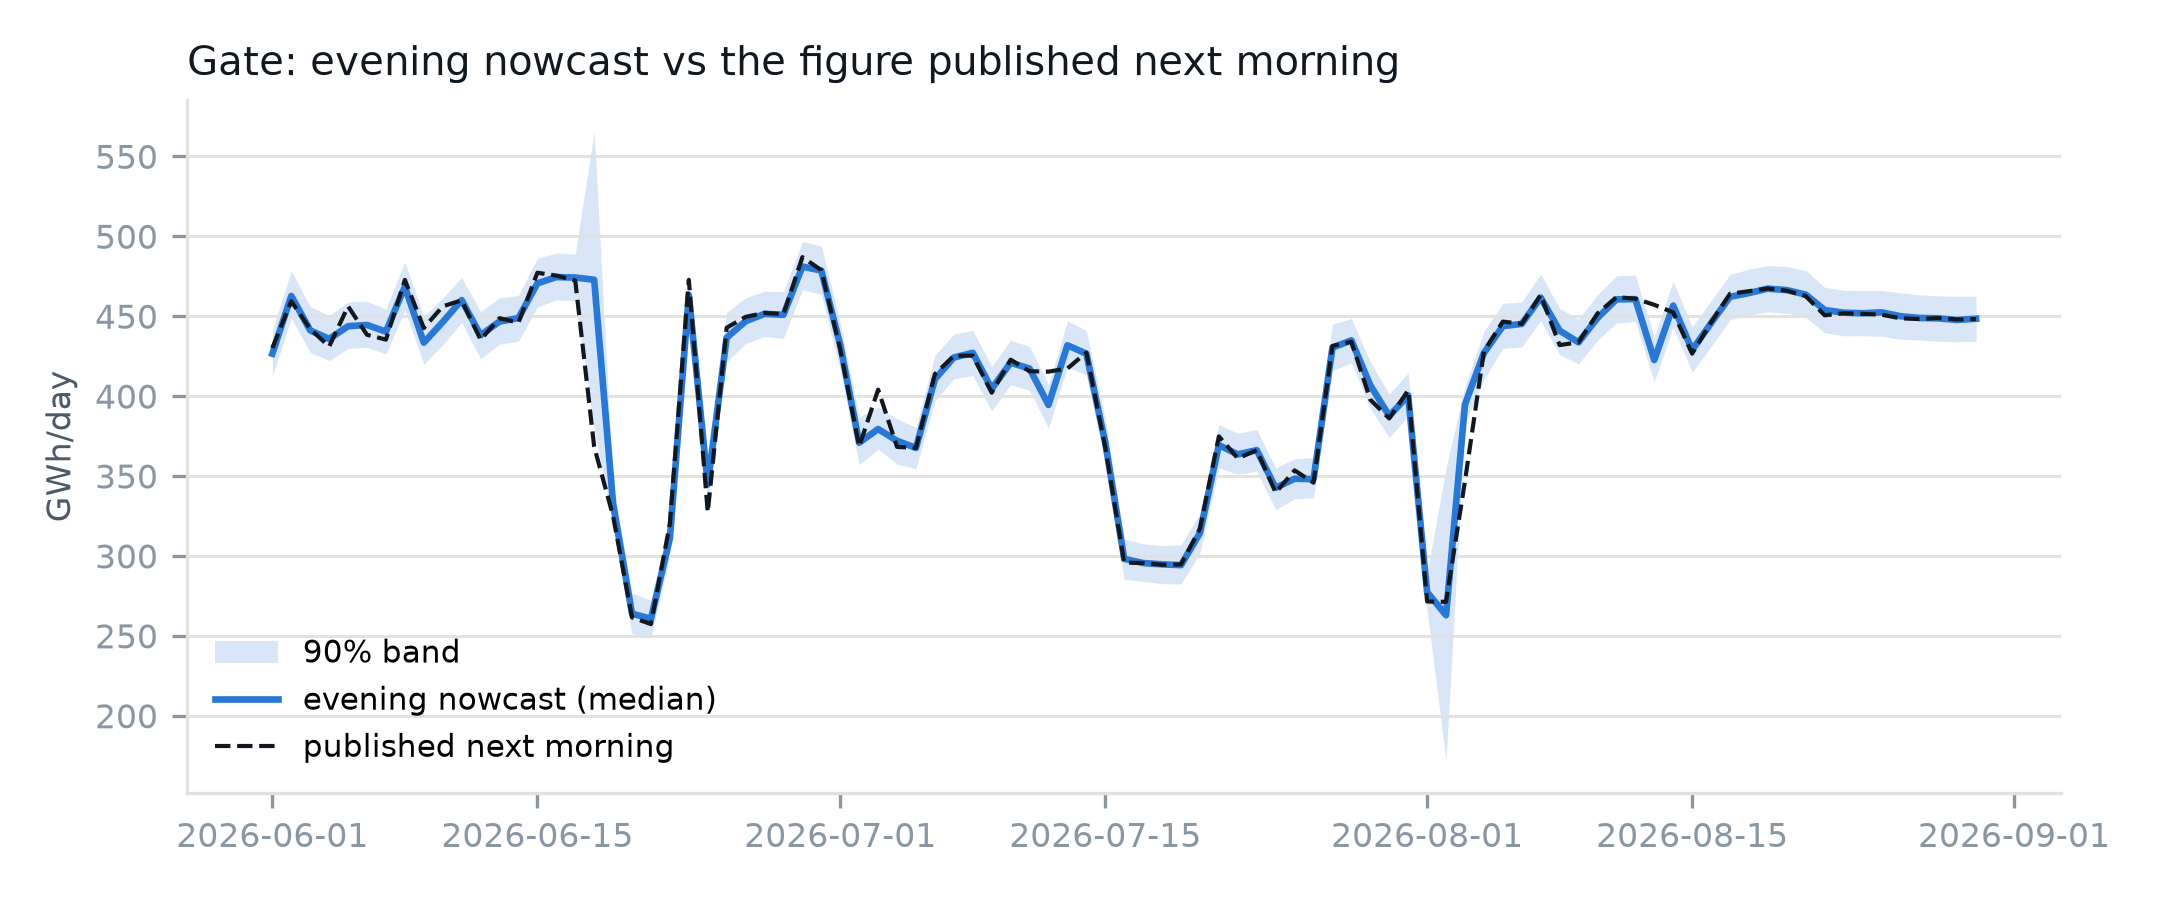
\includegraphics[width=\linewidth]{figures/fig_nowcast_bands.png}
\caption{Gate, June--August 2026: the evening nowcast (with 90\% band)
against the figure published the next morning; the band widens exactly at
the outage cliffs. \todo{caption polish.}}
\end{figure}
\begin{table}[h]\centering\small
\begin{tabular}{lcccccc}
\toprule
Terminal & H0 & H1 (midday) & H2 (evening) & persistence & nominations & cov90 (conf.) \\
\midrule
Gate & 20.7 & 8.4 & \textbf{4.5} & 20.6 & 63.0 & 0.92 \\
Eems & 15.3 & 4.4 & \textbf{2.1} & 15.1 & 35.8 & 0.93 \\
Zeebrugge & 47.1 & 32.0 & \textbf{24.3} & 47.1 & 120.3 & 0.87 \\
Dunkerque & 29.9 & -- & -- & 29.8 & 225.1 & 0.90 \\
Grain & 19.6 & -- & -- & 19.7 & -- & 0.89 \\
South Hook & 18.1 & -- & -- & 17.6 & -- & 0.91 \\
\bottomrule
\end{tabular}
\caption{MAE (GWh/d), 821 walk-forward days per terminal, 2024-06--2026-08;
bootstrap reference filter with bridge observations and adaptive-conformal
bands. \todo{add the RBPF column (500 particles, 15$\times$ faster,
comparable intraday, $p(\text{idle})$ output); describe horizons and the
leak-freedom of every fit.}}
\end{table}
\todo{Discussion: H0 ties persistence \emph{because} nominations are
empirically worse than persistence and are rejected by the fitted weight —
a data finding, not a modelling failure. Calibration: raw vs conformal,
Gibbs--Cand\`es guarantee and its marginal-only nature.}

\section{A physical stress index}
\begin{figure}[t]\centering
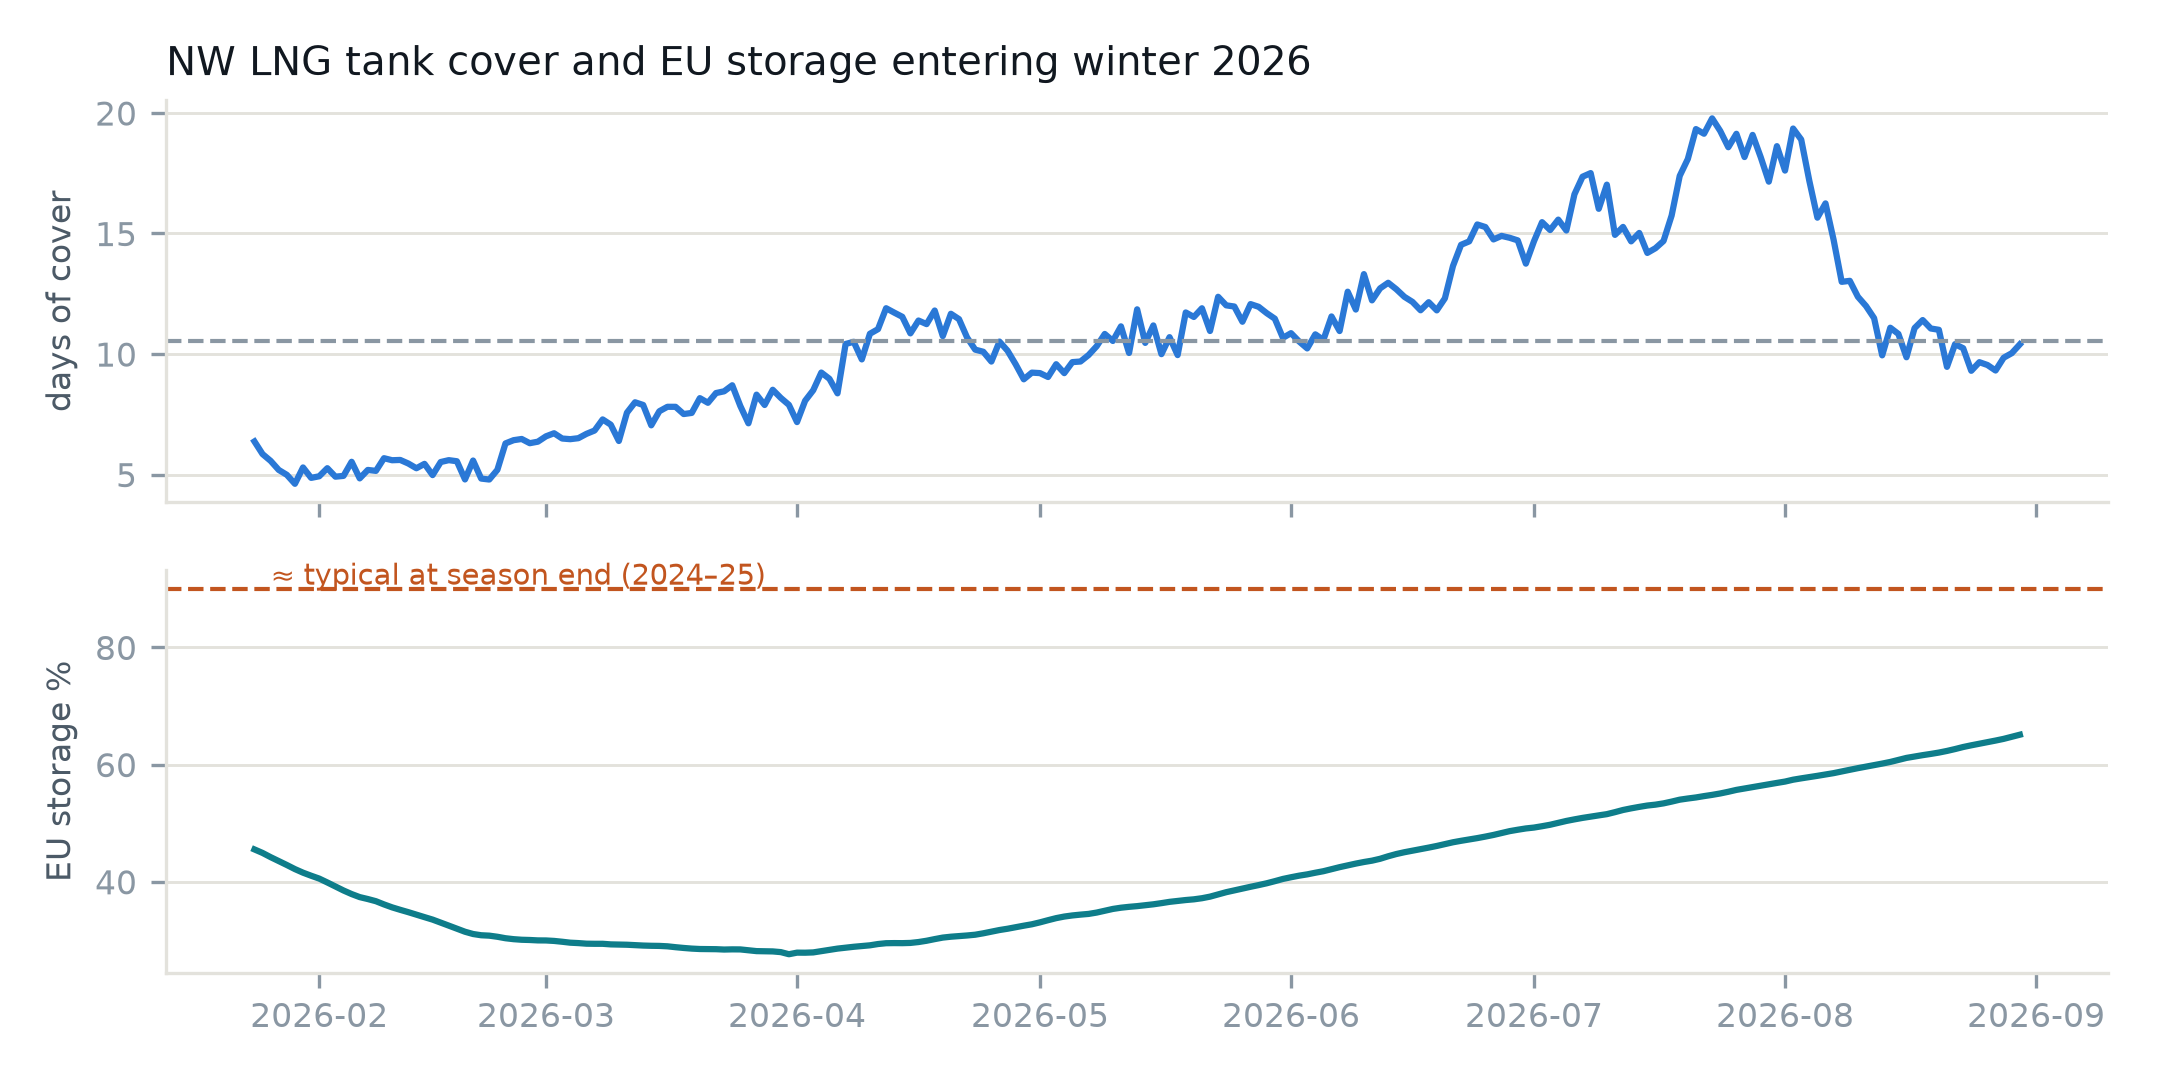
\includegraphics[width=\linewidth]{figures/fig_cover.png}
\caption{Days-of-cover and EU storage fullness entering winter 2026.
\todo{caption polish.}}
\end{figure}
\todo{Define days-of-cover; report the in-sample horse race — storage-\%
alone AUC 0.77--0.80 on TTF q97.5 spikes, $+$cover 0.85 (SAP: 0.62
$\to$ 0.73) — and give the caveats their own paragraph: in-sample
thresholds, overlapping windows, two winters, seasonal confounding
signatures in two components; specify the pre-registered out-of-sample
design for winter 2026--27 (storage entered September at 65\% vs
$\sim$90\% typical — the test will run live). Ship-pipeline layer:
departures/chokepoints/berths sampling design and why mid-ocean satellite
AIS is out of scope.}

\section{Economic content: a bounded null}
\todo{The event study: ordinary daily surprises ($\sigma \approx 109$ GWh)
move front-month TTF $\le 0.16\%$ same-day, $|t| < 1$ over 564 trading
days — a bound, consistent with damped-arbitrage structure; implications
for where value can live (prompt products, tails, conditional windows).}

\section{Limitations}
\todo{Own every weakness first: no historical satellite AIS (forward-only
ship layer); Zeebrugge residual miscalibration; cov50 width; UK intraday
horizons forward-only; stress study not yet out-of-sample; monetization
honesty (ICE TTF granularity vs a student account).}

\section*{Reproducibility}
All code, the snapshot archives, and every table's generating script are at
\url{https://github.com/solwilliams6305/LNG-send-out-nowcasting}. Data
sources are credited per their terms (GIE ALSI/AGSI as data source; ENTSOG;
National Gas; aisstream.io). \todo{pin commit hash at submission.}

\begin{thebibliography}{9}
\todo{Populate from the memo's reference list: Gibbs \& Cand\`es 2021/2024;
Zaffran et al.\ 2022; Sch\"on--Gustafsson--Nordlund 2005; Lindsten--Jordan--
Sch\"on 2014; Yu 2010 + JRSS-C 2025 zero-inflated HSMM; the AIS
destination-quality papers; the MIRP survey; LNG arbitrage economics.}
\end{thebibliography}
\end{document}
